\section*{Minimal system}

In this exercise, you will implement a standalone system with your own startup code.

\begin{enumerate}[itemsep=0pt]
    \item Create project without CMSIS Core and Device.
    \item Create a \(\texttt{start.c}\) file as discussed in the lab session.
    \item Add two files supplied with this assignment:
        \begin{itemize}
            \item \(\texttt{linear.c}\): Implements integer \(y = mx + c\), where \(m\) and \(c\) are 32-bit constants.
            \item \(\texttt{main.c}\): Calls \(\texttt{linear()}\) with different values of \(x\).
        \end{itemize}
    \item Fill in the following table.
        Specify the type to be one of:
        function, read-only data, initialized data, uninitialized data, local data.
\end{enumerate}

\subsection*{Solution}

\begin{table}[htbp]
    \centering
    \documentclass[border=3pt]{standalone}
\usepackage{tikz}

\begin{document}
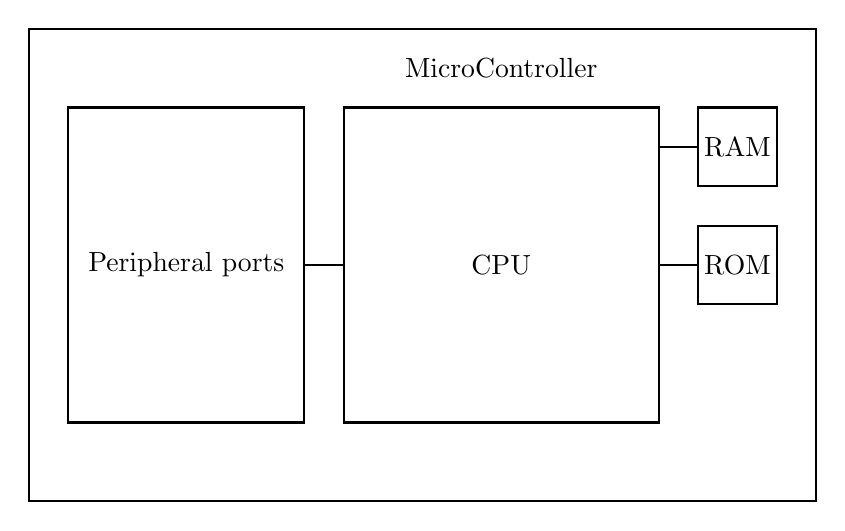
\begin{tikzpicture}

    \draw[thick] (0, 0) rectangle (10, 6);

    \draw[thick] (0.5, 1) rectangle (3.5, 5);
    \node at (2, 3) {Peripheral ports};

    \draw[thick] (4, 1) rectangle (8, 5);
    \node at (6, 3) {CPU};

    \draw[thick] (8.5, 4) rectangle (9.5, 5);
    \node at (9, 4.5) {RAM};

    \draw[thick] (8.5, 2.5) rectangle (9.5, 3.5);
    \node at (9, 3) {ROM};

    \draw[thick] (3.5, 3) -- (4, 3);
    \draw[thick] (8, 4.5) -- (8.5, 4.5);
    \draw[thick] (8, 3) -- (8.5, 3);

    \node at (6, 5.5) {MicroController};

\end{tikzpicture}
\end{document}

\end{table}
